\documentclass[12pt]{article}
\usepackage[margin=1in]{geometry}
\usepackage[all]{xy}
\usepackage{color}
\usepackage{enumerate}
\usepackage{amsmath,amsthm,amssymb,color,latexsym}
\usepackage{geometry}        
\usepackage{graphicx}
\usepackage{caption}
\usepackage{float}
\usepackage{stfloats}
\newtheorem{parter}{Part}
\newtheorem*{efficiency}{Efficiency}
\newtheorem*{example}{Example}
\newtheorem{step}{Step}
\newenvironment{solution}


\begin{document}
\noindent ECS 174 Spring 2020 \ (05/11)\hfill Problem Set \#2\\
Bingwei Wang \ 914683636\\
Nan Chen \ 915218152

\hrulefill

\begin{parter}
\end{parter}
    
\begin{solution}
    \begin{itemize}
        \item [(1)]We believe that the grouping algorithm graph-cuts, would be the most appropriate grouping algorithm to recover the model parameter hypotheses from the continuous vote space. The reason is that each edge of it has its own affinity weight, and pixels are linked in pairs. Additionally, graph-cuts connect shapes on edges with high affinity while mean shift and k-means does not, which works well when shapes are defined by boundary points in Hough Transform. \\
        \\ But here comes a problem which we find mean-shifts might have better performance. Graph-cuts use a pixel-based energy function to compute the similarity of neighboring pixels, while in a continuous space we cannot count the number of points or their neighbors, so this would not work. For mean-shift, it is non-parametric and does not segment the vote space. We do not need to discretize of the vote space in the mean-shift algorithm because the algorithm itself already does it.\\        
        \\ We do not choose k-means because in continuous vote space, it is hard(impossible) to select parameter k.
        \item [(2)]After using K-means to cluster those points into two groups, we will have two center points for outputs in two clusters. Each center point will be randomly positioned at the beginning. After that, new positions of two center points will be updated by calculating the least squared Euclidean distance from feature points in its own cluster. The process will keep repeated until feature points are divided equally in two groups, belonging to those two center points, which means half points will be close to one center point, and half will be close to the other center point.
        \item [(3)]Variables and Pseudocode:
        \begin{figure}[H]
            \centering
            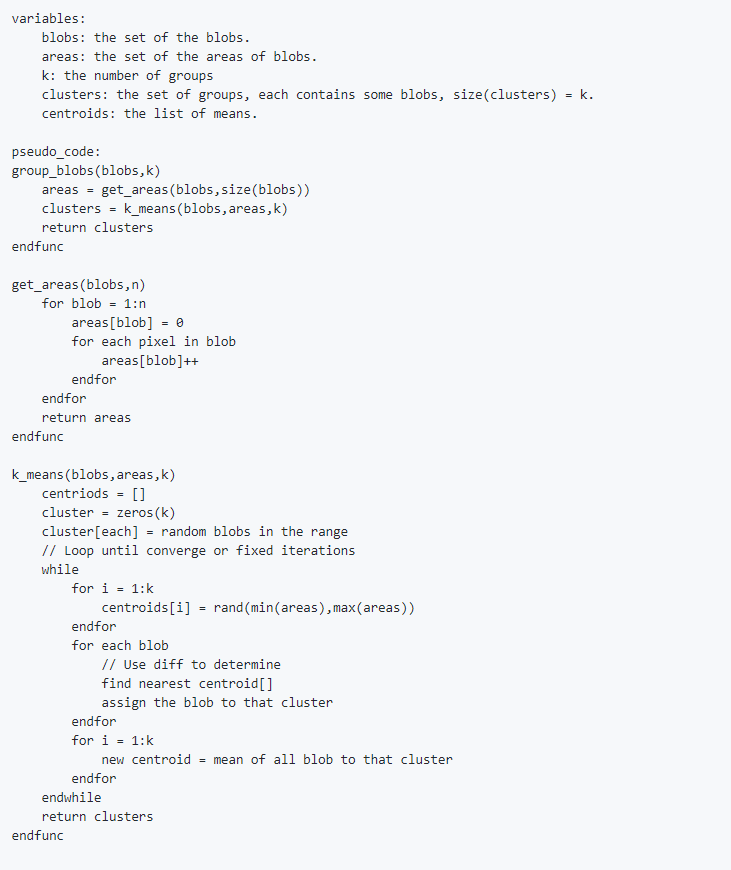
\includegraphics[width=16cm, height=20cm]{../pseudocode.png}
        \end{figure}
        {$\square$}
    \end{itemize}
\end{solution}
\clearpage
\begin{parter}
\end{parter}
    
\begin{solution}
    \begin{itemize}
        \item [(a)]The code is written in file \textbf{get\_correspondences.m}. The function has two inputs of two images and the number of points the user wants to pick. The outputs are two 2 x N point matrices of selected points.
        \item [(b)]The code is written in file \textbf{computeH.m}.
        \item [(c)]The code is written in file \textbf{warpImage.m}.
        \item [(d)]Images:
        \begin{figure}[H]
            \centering
            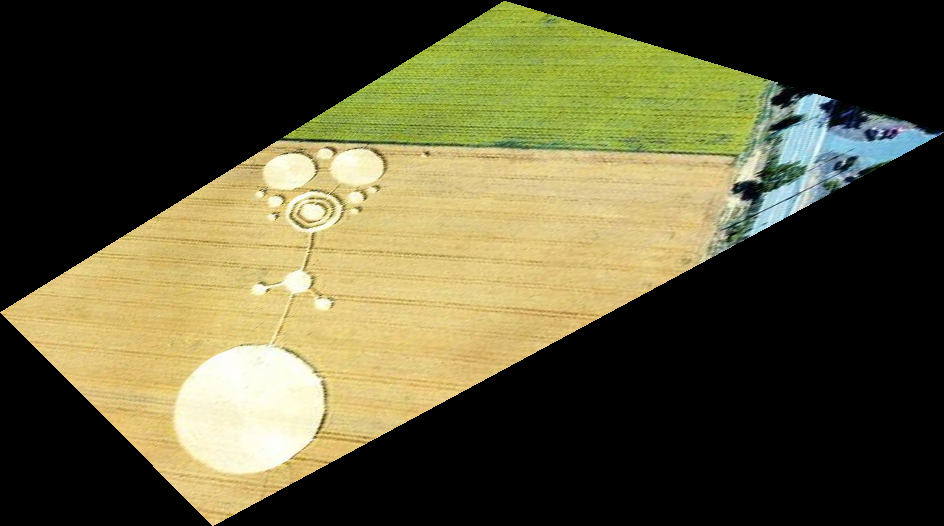
\includegraphics[width=16cm, height=10cm]{../cropwarp.png}
            \caption{crop\_warp}
        \end{figure}
        \begin{figure}[H]
            \centering
            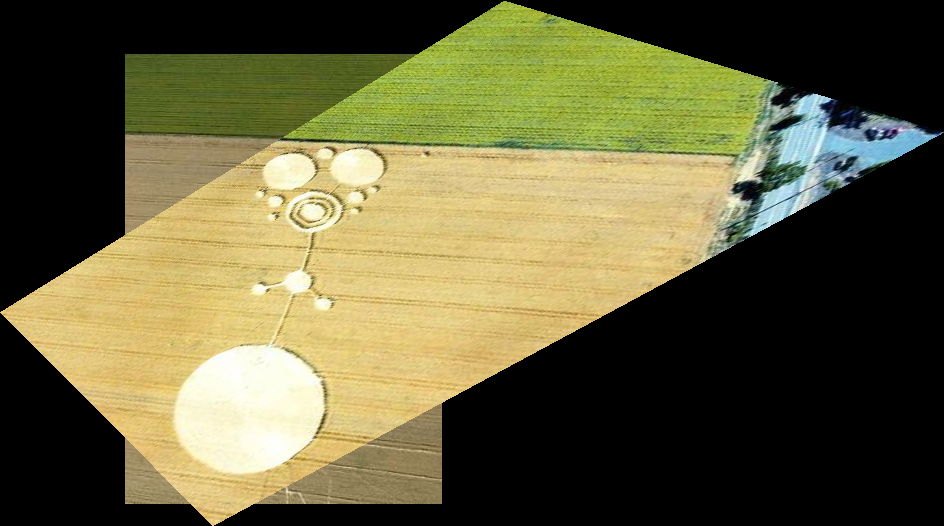
\includegraphics[width=16cm, height=10cm]{../cropmos.png}
            \caption{crop\_merge}
        \end{figure}
        \begin{figure}[H]
            \centering
            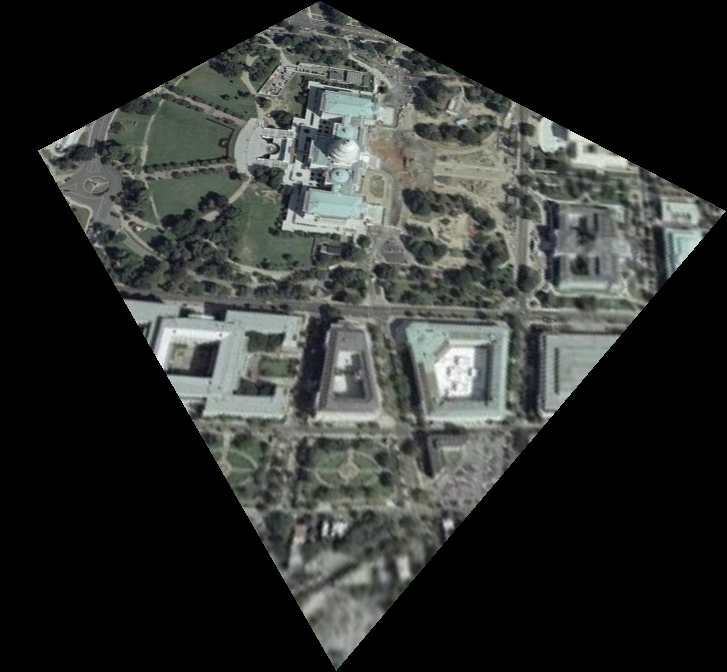
\includegraphics[width=10cm, height=12cm]{../wdcwarp.png}
            \caption{wdc\_warp}
        \end{figure}
        \begin{figure}[H]
            \centering
            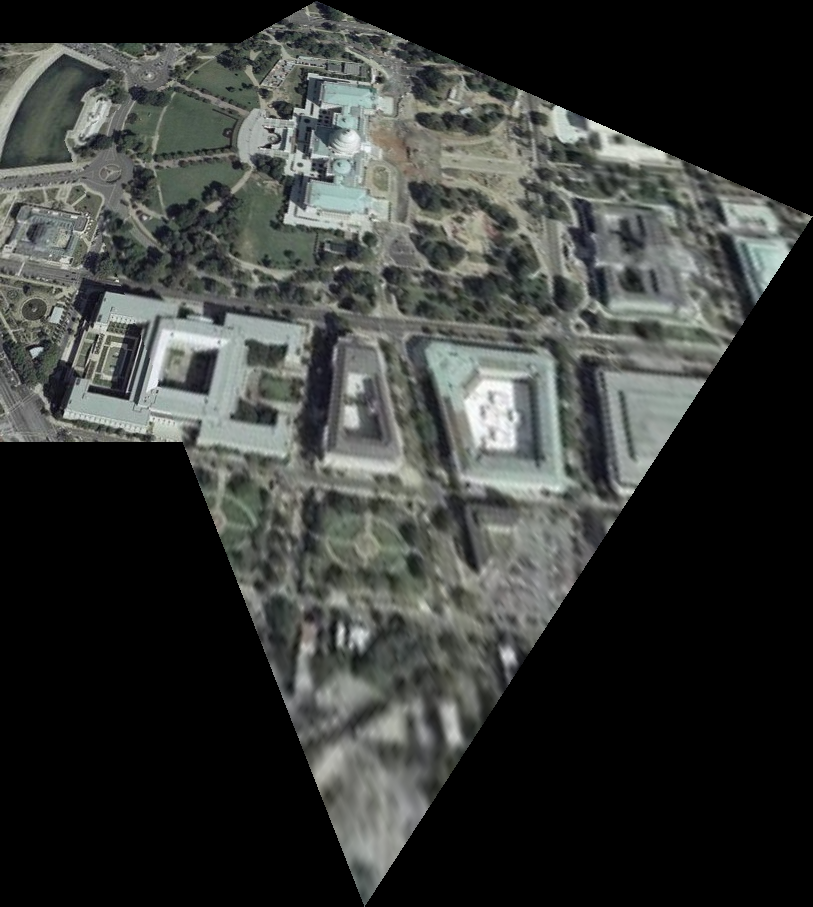
\includegraphics[width=10cm, height=12cm]{../wdcmos.png}
            \caption{wdc\_merge}
        \end{figure}
        The data points1 and points2 are saved in the file \textbf{points.m}.
        \item [(e)] Images:
        \begin{figure}[htbp]
            \centering
            \begin{minipage}[t]{0.48\textwidth}
            \centering
            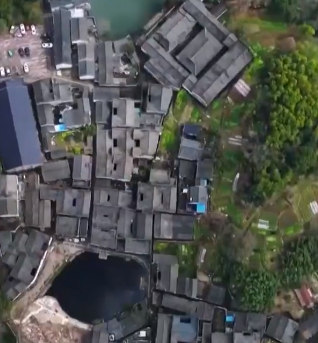
\includegraphics[width=5cm, height=6cm]{../town1.png}
            \caption{town\_source\_1}
            \end{minipage}
            \begin{minipage}[t]{0.48\textwidth}
            \centering
            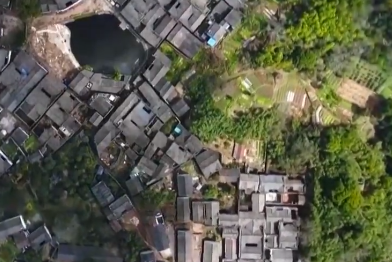
\includegraphics[width=7cm, height=5cm]{../town2.png}
            \caption{town\_source\_2}
            \end{minipage}
        \end{figure}
        \begin{figure}[H]
            \centering
            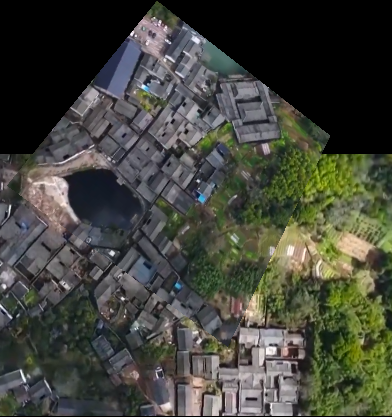
\includegraphics[width=11cm, height=12cm]{../townmos.png}
            \caption{town\_mosic}
        \end{figure}
        Source: https://www.bilibili.com/bangumi/play/ep264278.
        \\
        \\
        Another example (can be omitted):
        \begin{figure}[htbp]
            \centering
            \begin{minipage}[t]{0.48\textwidth}
            \centering
            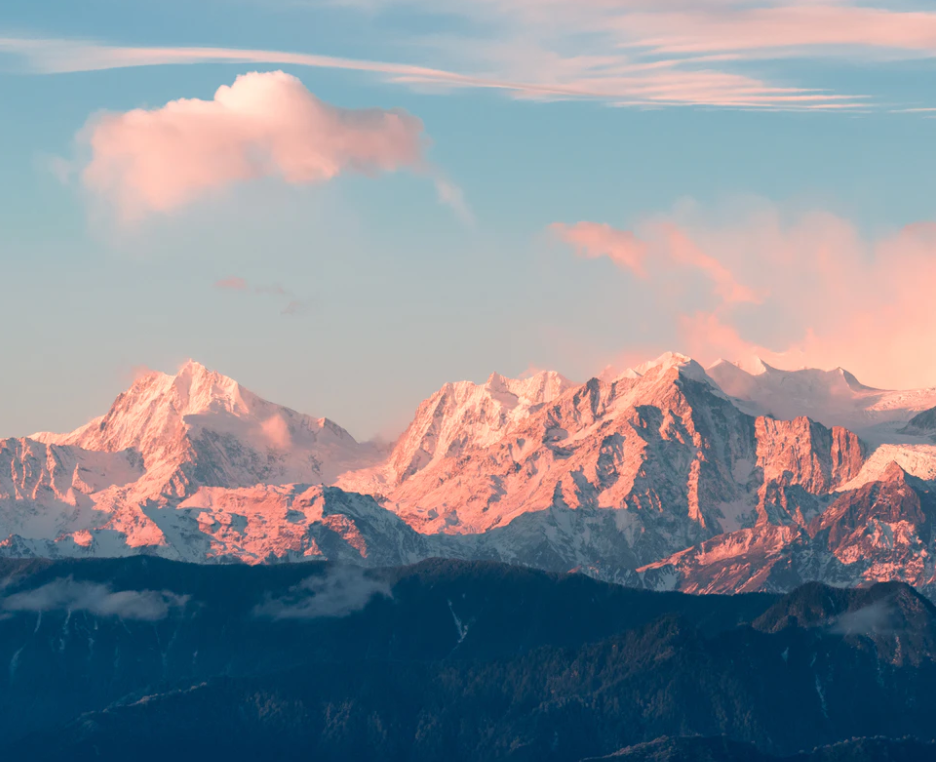
\includegraphics[width=6cm, height=7cm]{../mountain1.png}
            \caption{mountain\_source\_1}
            \end{minipage}
            \begin{minipage}[t]{0.48\textwidth}
            \centering
            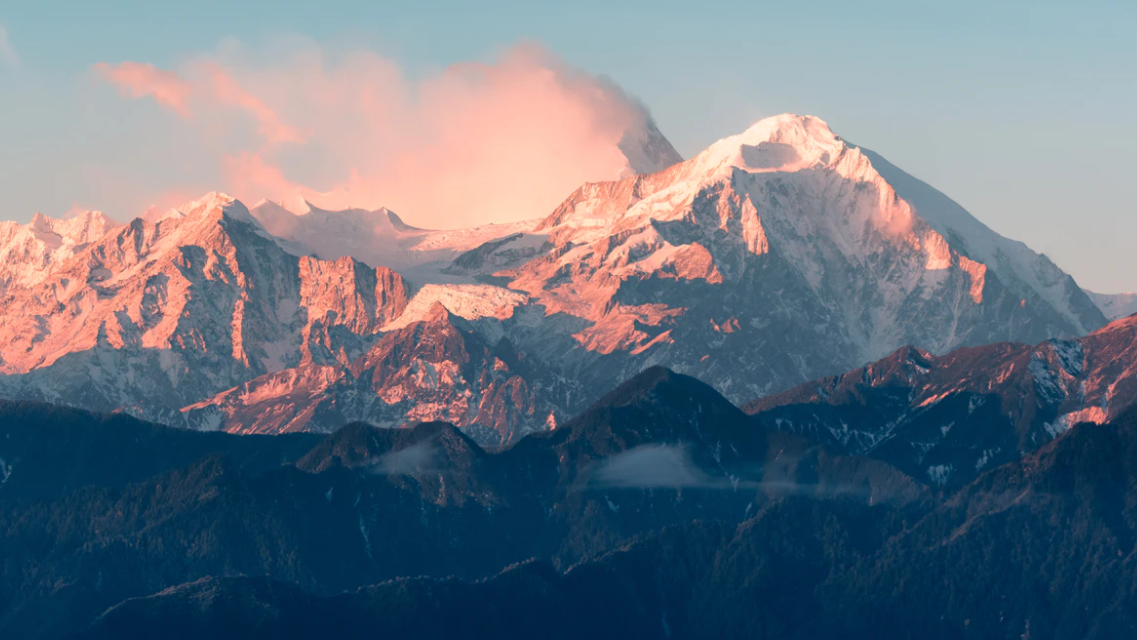
\includegraphics[width=7cm, height=5cm]{../mountain2.png}
            \caption{mountain\_source\_2}
            \end{minipage}
        \end{figure}
        \begin{figure}[H]
            \centering
            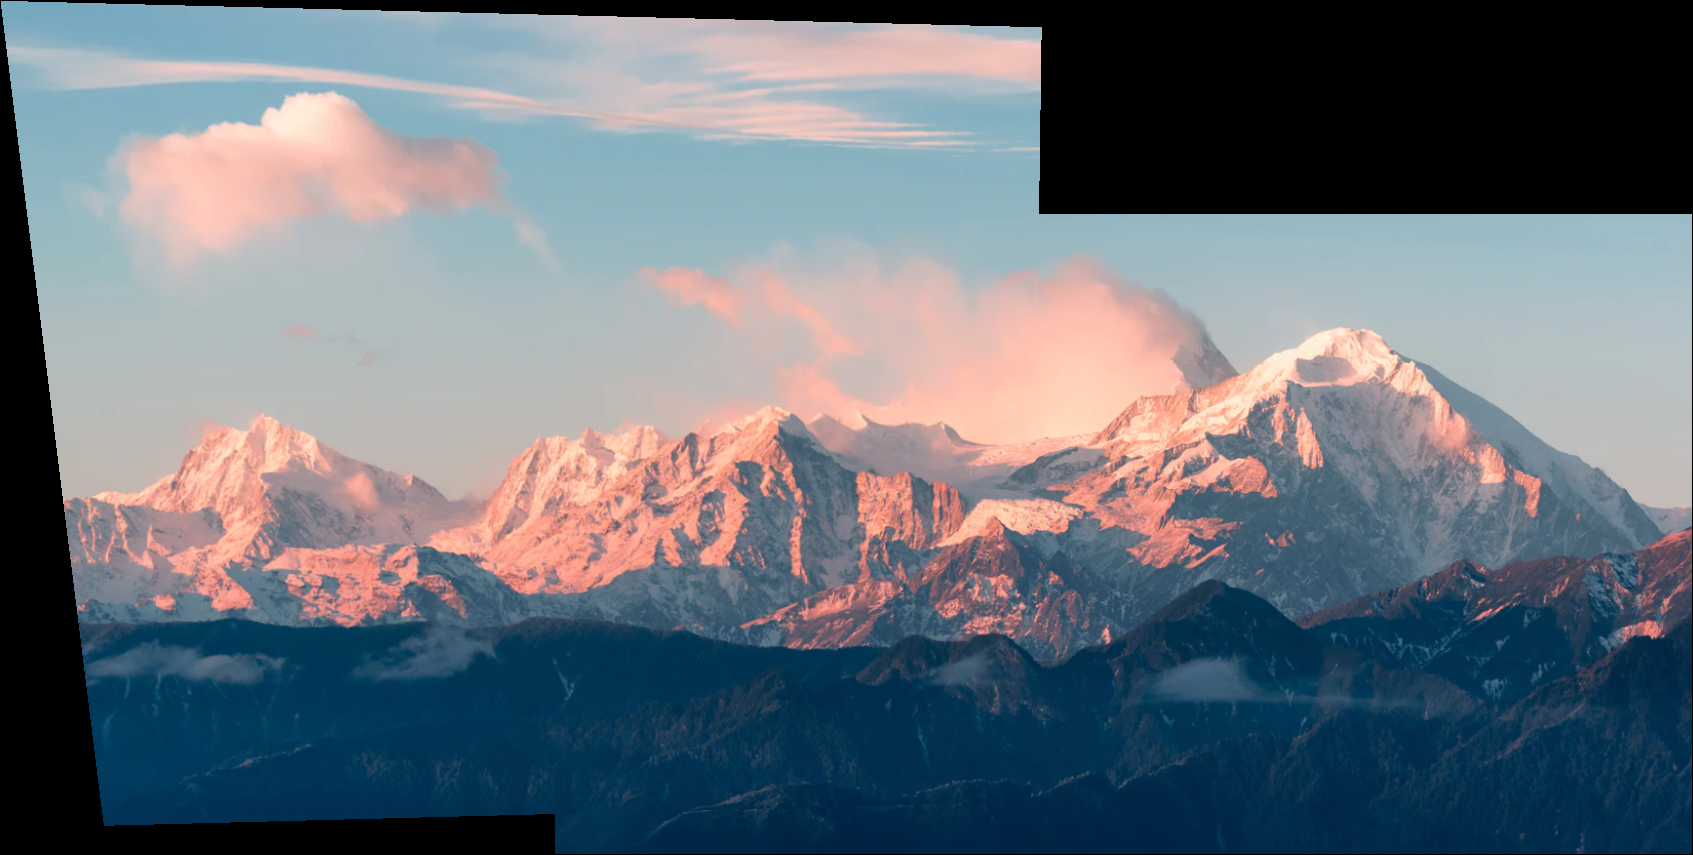
\includegraphics[width=15cm, height=10cm]{../mountainmos.png}
            \caption{mountain\_mosic}
        \end{figure}
        Source: https://unsplash.com/photos/Y8lCoTRgHPE.
        \item [(f)] Images:
        \begin{figure}[H]
            \centering
            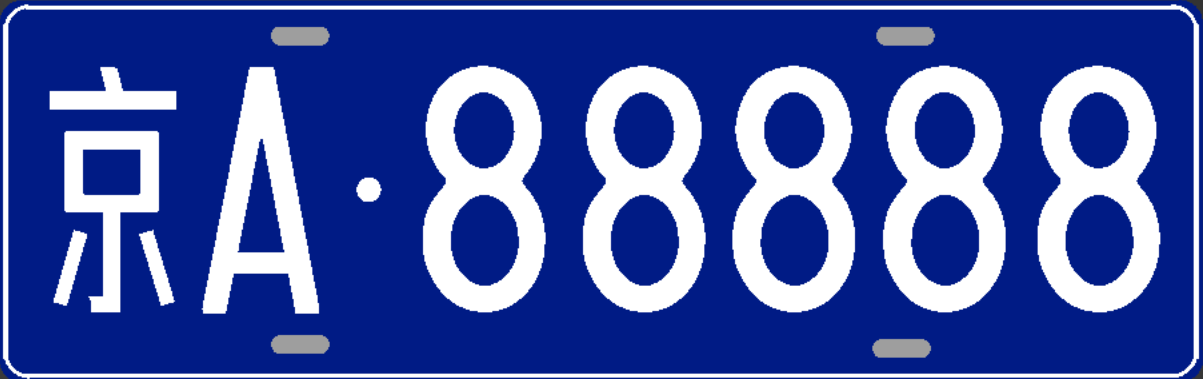
\includegraphics[width=15cm, height=5cm]{../plate.png}
            \caption{plate}
        \end{figure}
        \begin{figure}[H]
            \centering
            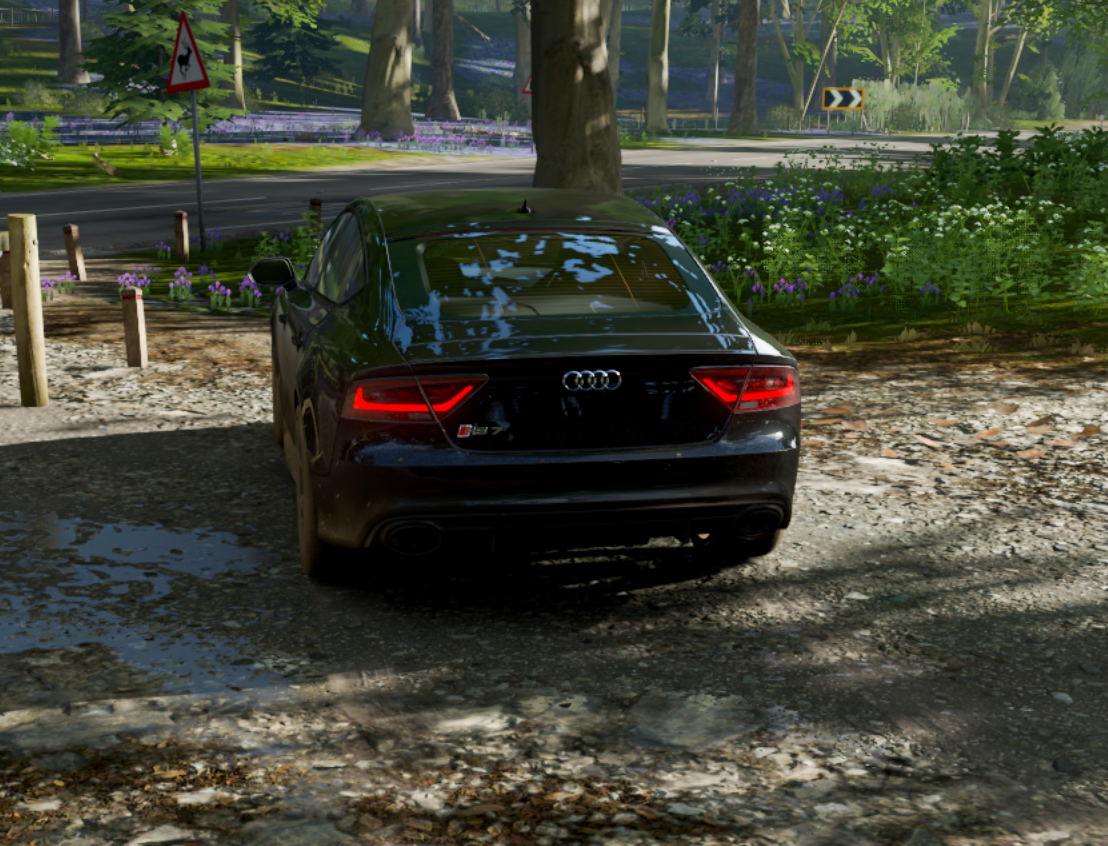
\includegraphics[width=15cm, height=12cm]{../car.png}
            \caption{car}
        \end{figure}
        \begin{figure}[H]
            \centering
            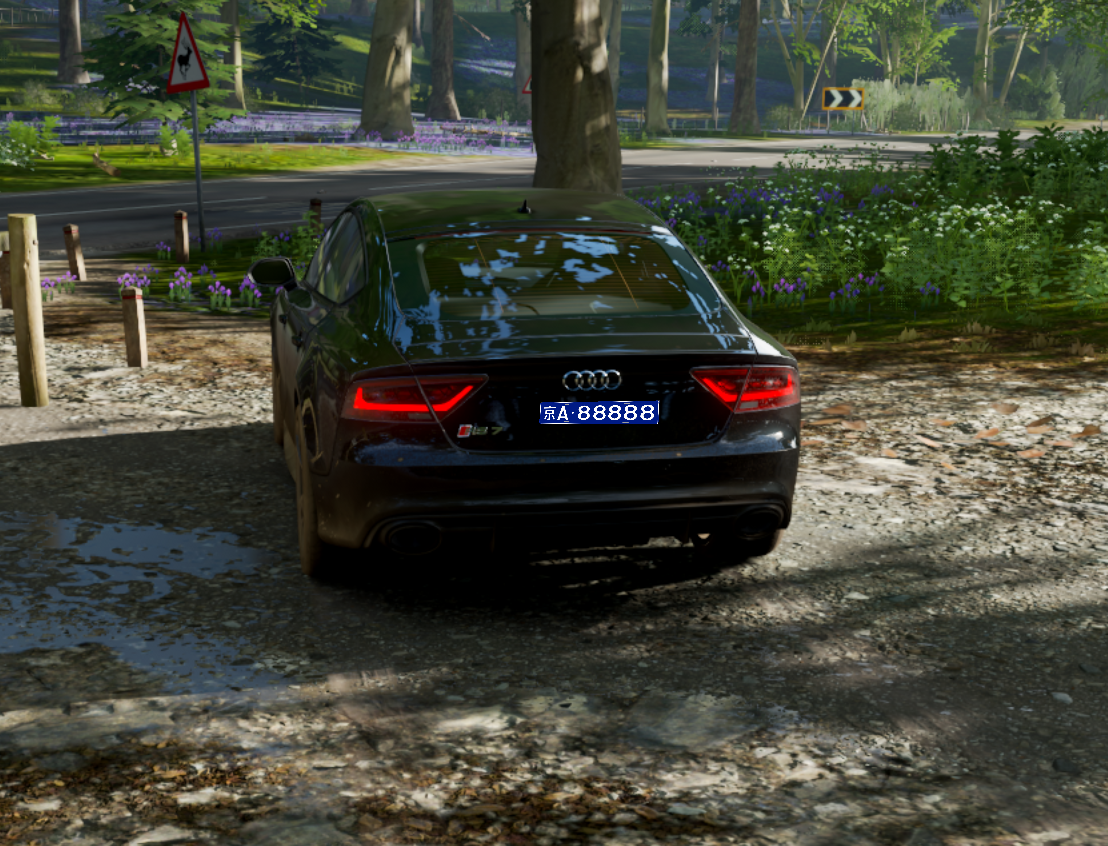
\includegraphics[width=15cm, height=12cm]{../carmos.png}
            \caption{car\_mosic}
        \end{figure}
        Source: ScreenShots from Game Forza Horizon4.\\
        Take the license plate picture, and mosic it on the car.
        {$\square$}
    \end{itemize}
\end{solution}

\begin{parter}
\end{parter}
    
\begin{solution}
    \begin{itemize}
        \item [(a)] Images:
        \begin{figure}[htbp]
            \centering
            \begin{minipage}[t]{0.48\textwidth}
            \centering
            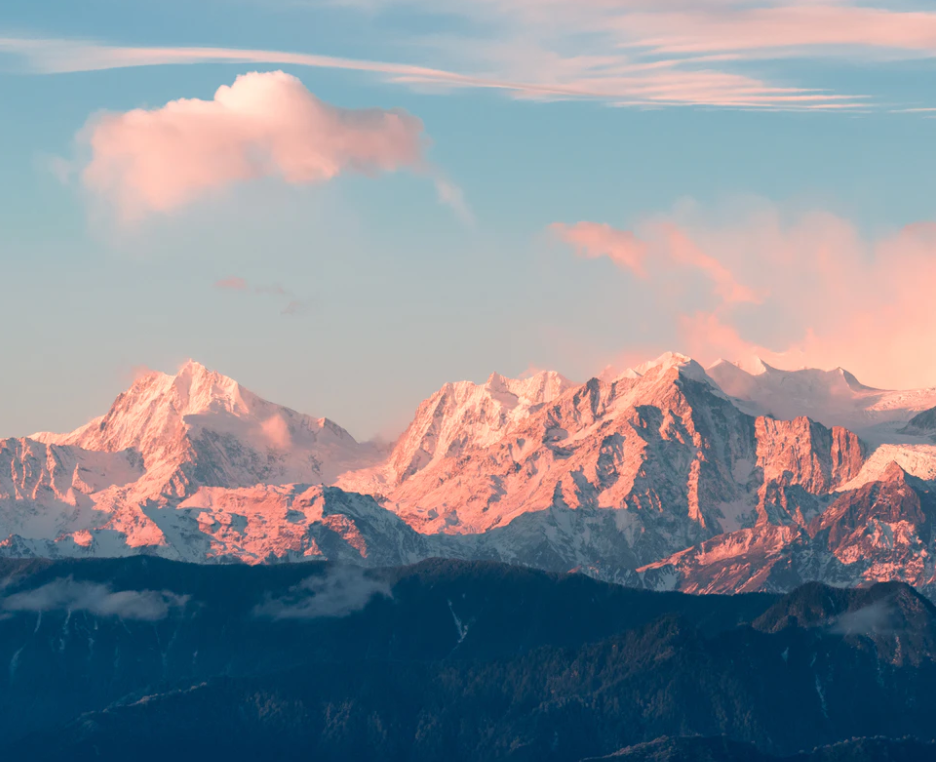
\includegraphics[width=6cm, height=7cm]{../mountain1.png}
            \caption{mountain\_source\_1}
            \end{minipage}
            \begin{minipage}[t]{0.48\textwidth}
            \centering
            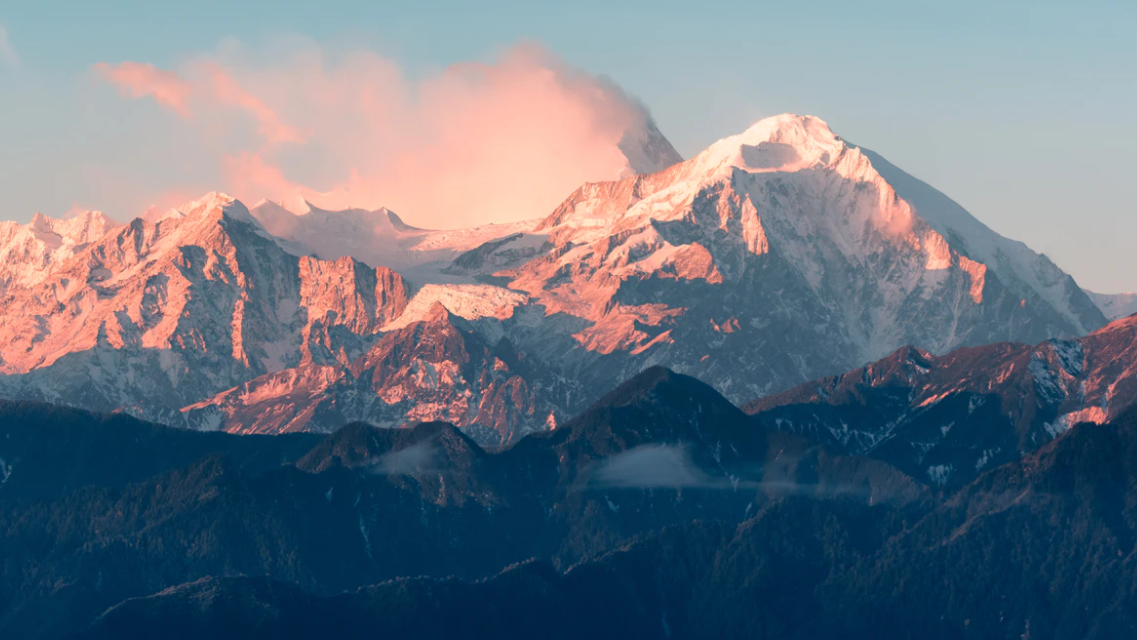
\includegraphics[width=7cm, height=5cm]{../mountain2.png}
            \caption{mountain\_source\_2}
            \end{minipage}
        \end{figure}
        \begin{figure}[htbp]
            \centering
            \begin{minipage}[t]{0.48\textwidth}
            \centering
            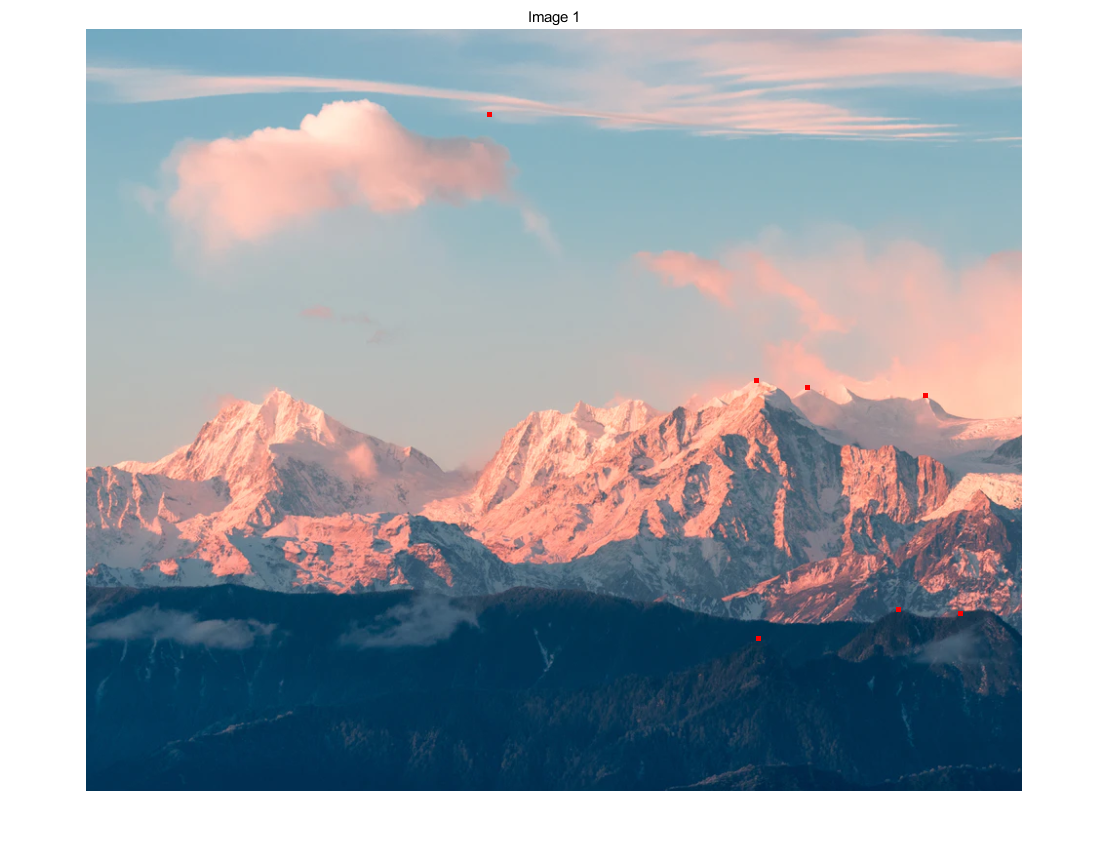
\includegraphics[width=6cm, height=7cm]{../mountain1_select.png}
            \caption{mountain\_select\_1}
            \end{minipage}
            \begin{minipage}[t]{0.48\textwidth}
            \centering
            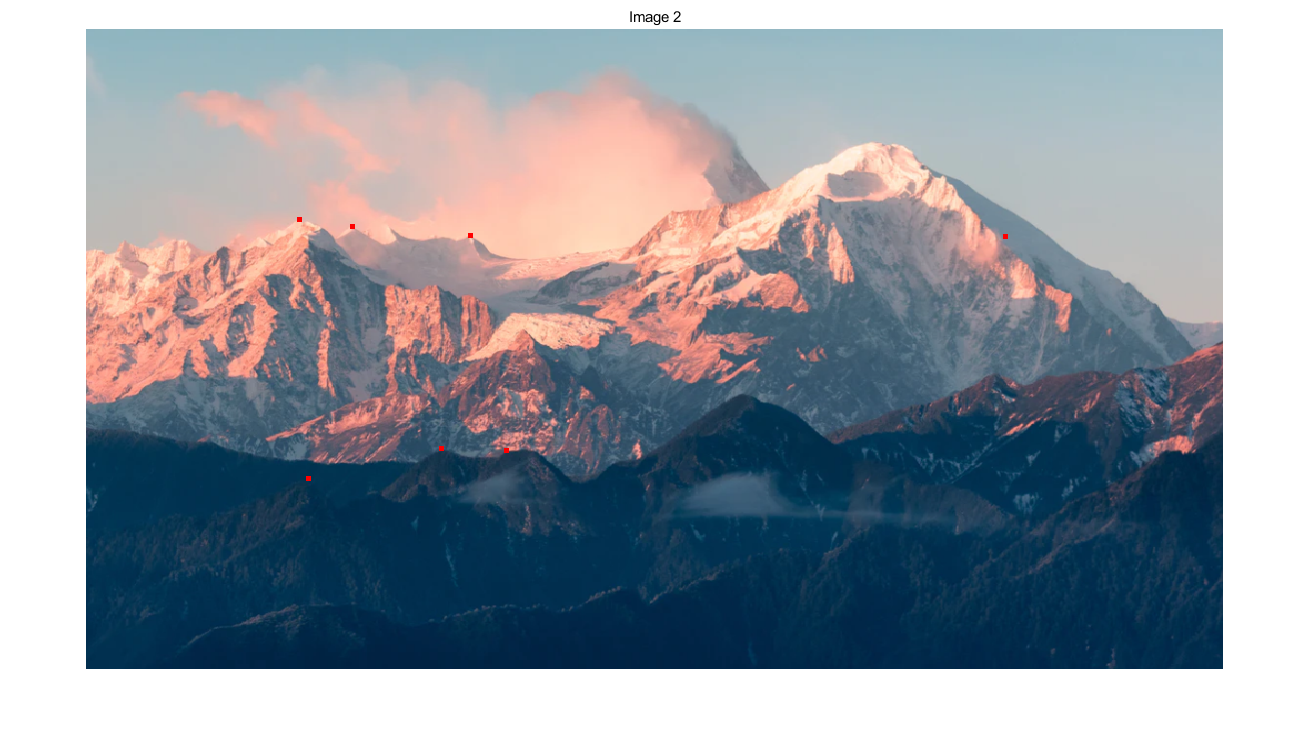
\includegraphics[width=7cm, height=5cm]{../mountain2_select.png}
            \caption{mountain\_select\_2}
            \end{minipage}
        \end{figure}
        \begin{figure}[H]
            \centering
            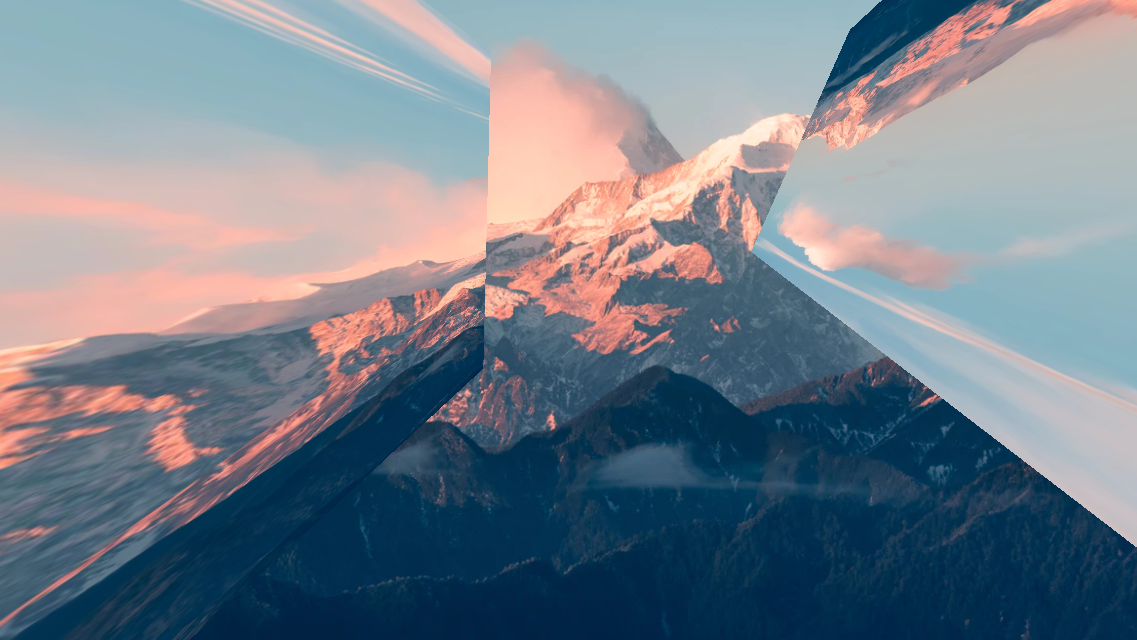
\includegraphics[width=15cm, height=10cm]{../mountainmos_O.png}
            \caption{mountain\_mosic\_original}
        \end{figure}
        \begin{figure}[H]
            \centering
            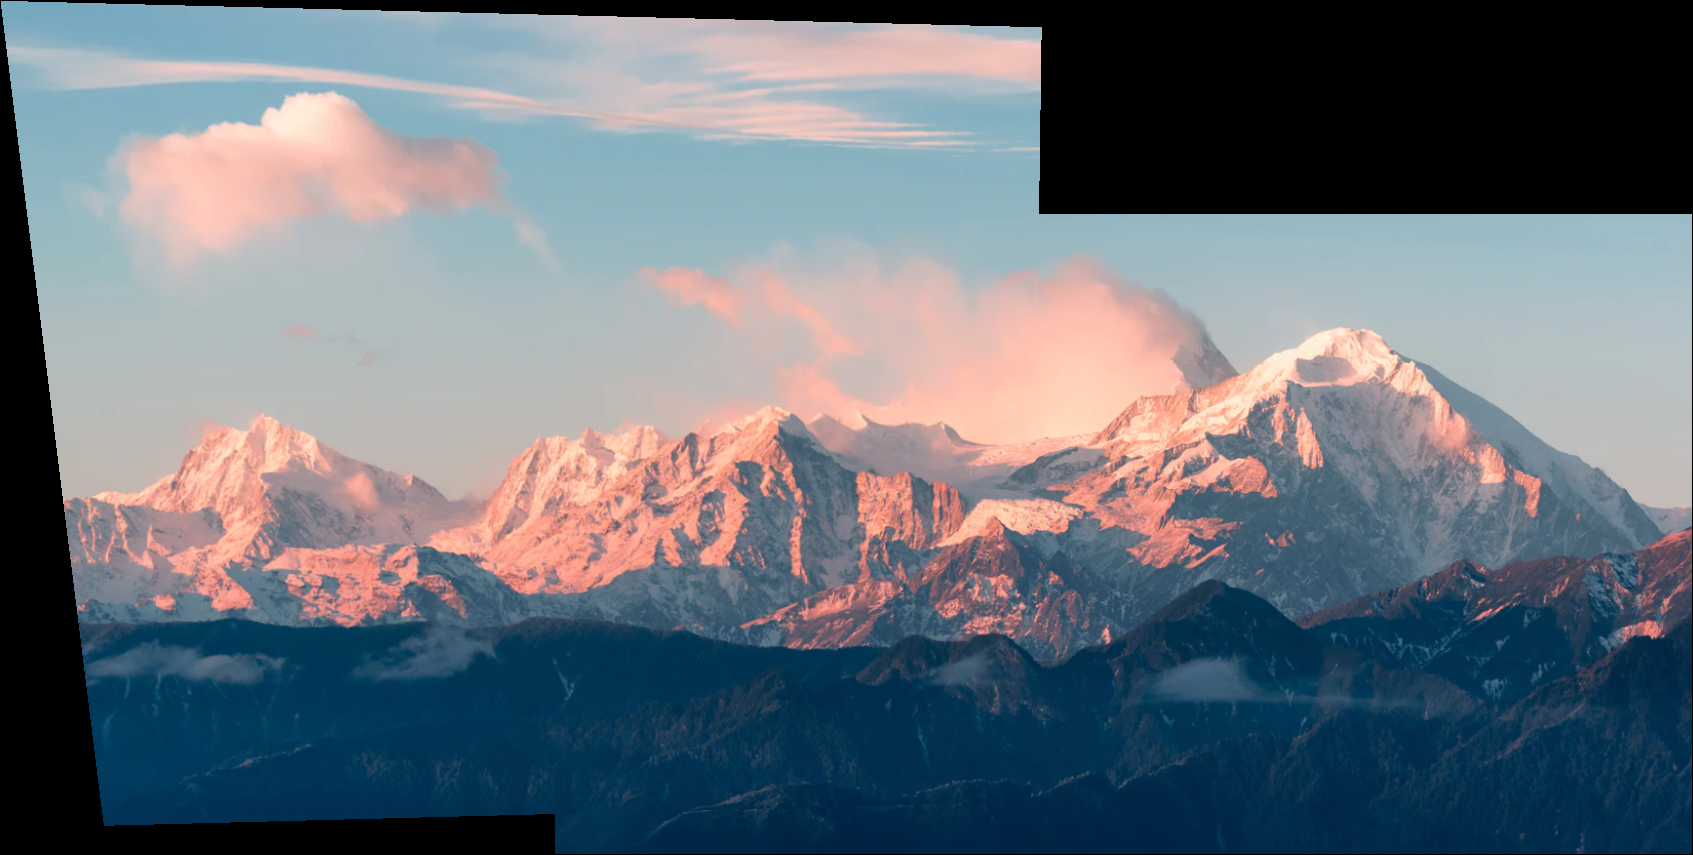
\includegraphics[width=15cm, height=10cm]{../mountainmos_R.png}
            \caption{mountain\_mosic\_RANSAC}
        \end{figure}
        Source: https://unsplash.com/photos/Y8lCoTRgHPE.\\
        \\
        Code: \textbf{RANSAC\_script.m} and \textbf{RANSAC.m}.\\
        \\
        Explanation: We implemented a new function \textbf{bestH = RANSAC(t1, t2)} to calculate the new H value using RANSAC algorithm.
        From Figure 16 and Figure 17, we can see there is one bad point selected. Thus, in Figure 18, the image
        is "broken" and no longer seems "stitch". In Figure 19, we use RANSAC method, and that can eliminate the bad point; therefore, gives us the correct stitch.\\
        \\
        Implementation: The user can use the script \textbf{RANSAC\_script.m} and change the image names to get results with RANSAC algorithm.
        \item [(b)] Images:
        \begin{figure}[H]
            \centering
            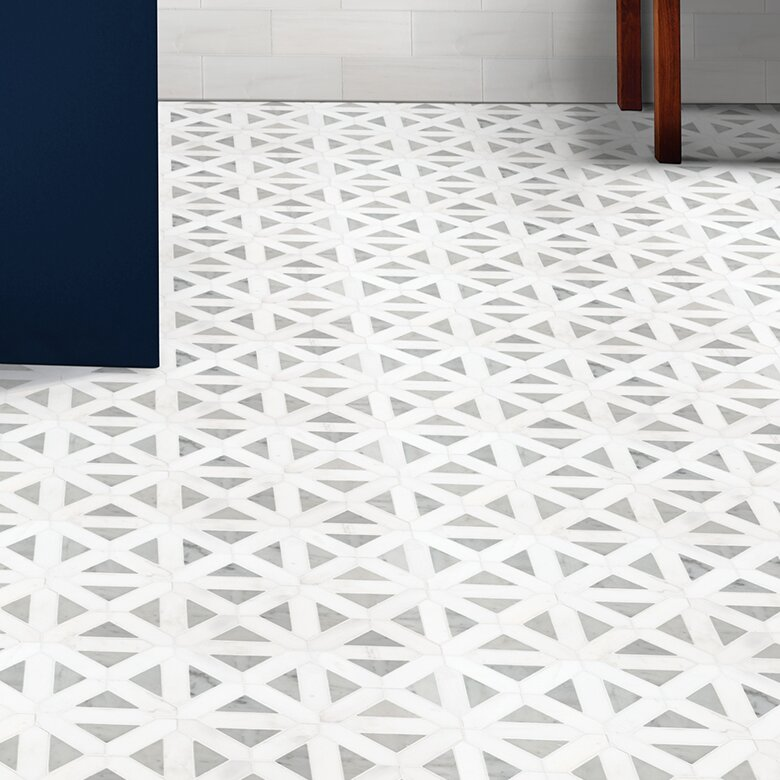
\includegraphics[width=15cm, height=12cm]{../tiles.jpg}
            \caption{tiles\_source}
        \end{figure}
        \begin{figure}[H]
            \centering
            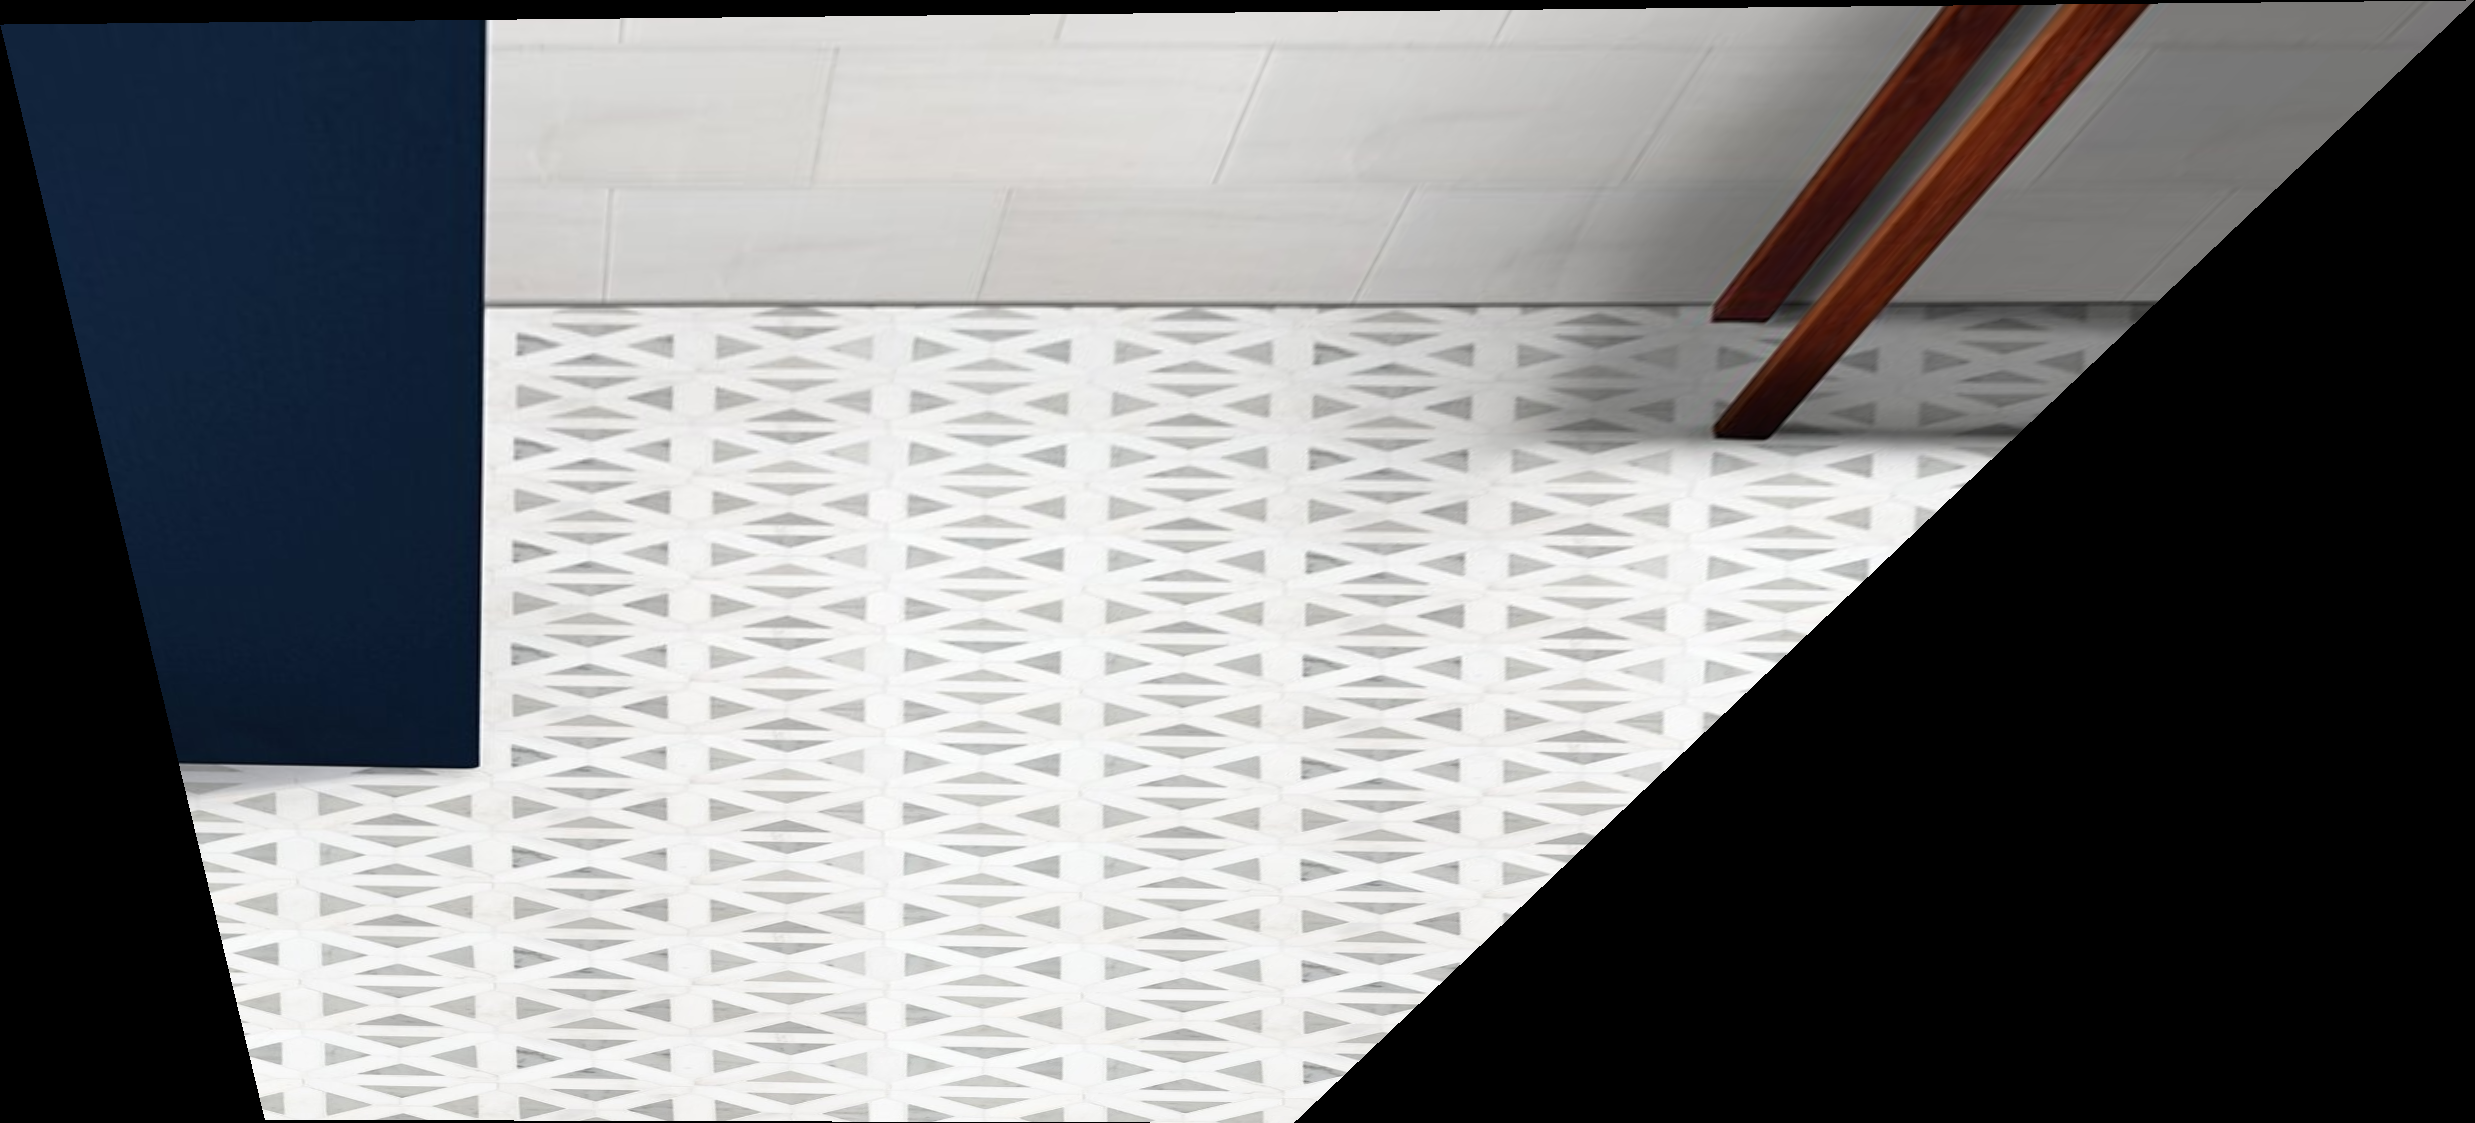
\includegraphics[width=15cm, height=12cm]{../tilesmos.png}
            \caption{tiles\_fronto}
        \end{figure}
        Source: https://www.wayfair.com/home-improvement/pdp/msi-bianco-dolomite-marble-mosaic-tile-mvp4112.html?piid=49665325.\\
        \\
        Code: \textbf{fronto\_script.m} and \textbf{get\_correspondences\_fronto.m}.\\
        \\
        Explanation: We revised the \textbf{get\_correspondences()} function to only get the four points of one image. Then, we use these four points
        as the first input points to compute H, and we selected the four corners of the image as the second input points to compute H. Lastly, as
        usual, we use the image twice and H to get the results. \\
        \\
        Implementation: The user can use the script \textbf{fronto\_script.m} and change the image name to get results. Either warp result or merge result
        is okay.
        {$\square$}
    \end{itemize}
\end{solution}

\end{document}